
%% bare_jrnl.tex
%% V1.4a
%% 2014/09/17
%% by Michael Shell
%% see http://www.michaelshell.org/
%% for current contact information.
%%
%% This is a skeleton file demonstrating the use of IEEEtran.cls
%% (requires IEEEtran.cls version 1.8a or later) with an IEEE
%% journal paper.
%%
%% Support sites:
%% http://www.michaelshell.org/tex/ieeetran/
%% http://www.ctan.org/tex-archive/macros/latex/contrib/IEEEtran/
%% and
%% http://www.ieee.org/

%%*************************************************************************
%% Legal Notice:
%% This code is offered as-is without any warranty either expressed or
%% implied; without even the implied warranty of MERCHANTABILITY or
%% FITNESS FOR A PARTICULAR PURPOSE! 
%% User assumes all risk.
%% In no event shall IEEE or any contributor to this code be liable for
%% any damages or losses, including, but not limited to, incidental,
%% consequential, or any other damages, resulting from the use or misuse
%% of any information contained here.
%%
%% All comments are the opinions of their respective authors and are not
%% necessarily endorsed by the IEEE.
%%
%% This work is distributed under the LaTeX Project Public License (LPPL)
%% ( http://www.latex-project.org/ ) version 1.3, and may be freely used,
%% distributed and modified. A copy of the LPPL, version 1.3, is included
%% in the base LaTeX documentation of all distributions of LaTeX released
%% 2003/12/01 or later.
%% Retain all contribution notices and credits.
%% ** Modified files should be clearly indicated as such, including  **
%% ** renaming them and changing author support contact information. **
%%
%% File list of work: IEEEtran.cls, IEEEtran_HOWTO.pdf, bare_adv.tex,
%%                    bare_conf.tex, bare_jrnl.tex, bare_conf_compsoc.tex,
%%                    bare_jrnl_compsoc.tex, bare_jrnl_transmag.tex
%%*************************************************************************


% *** Authors should verify (and, if needed, correct) their LaTeX system  ***
% *** with the testflow diagnostic prior to trusting their LaTeX platform ***
% *** with production work. IEEE's font choices and paper sizes can       ***
% *** trigger bugs that do not appear when using other class files.       ***                          ***
% The testflow support page is at:
% http://www.michaelshell.org/tex/testflow/



\documentclass[journal]{IEEEtran}
%
% If IEEEtran.cls has not been installed into the LaTeX system files,
% manually specify the path to it like:
% \documentclass[journal]{../sty/IEEEtran}





% Some very useful LaTeX packages include:
% (uncomment the ones you want to load)


% *** MISC UTILITY PACKAGES ***
%
%\usepackage{ifpdf}
% Heiko Oberdiek's ifpdf.sty is very useful if you need conditional
% compilation based on whether the output is pdf or dvi.
% usage:
% \ifpdf
%   % pdf code
% \else
%   % dvi code
% \fi
% The latest version of ifpdf.sty can be obtained from:
% http://www.ctan.org/tex-archive/macros/latex/contrib/oberdiek/
% Also, note that IEEEtran.cls V1.7 and later provides a builtin
% \ifCLASSINFOpdf conditional that works the same way.
% When switching from latex to pdflatex and vice-versa, the compiler may
% have to be run twice to clear warning/error messages.






% *** CITATION PACKAGES ***
%
%\usepackage{cite}
% cite.sty was written by Donald Arseneau
% V1.6 and later of IEEEtran pre-defines the format of the cite.sty package
% \cite{} output to follow that of IEEE. Loading the cite package will
% result in citation numbers being automatically sorted and properly
% "compressed/ranged". e.g., [1], [9], [2], [7], [5], [6] without using
% cite.sty will become [1], [2], [5]--[7], [9] using cite.sty. cite.sty's
% \cite will automatically add leading space, if needed. Use cite.sty's
% noadjust option (cite.sty V3.8 and later) if you want to turn this off
% such as if a citation ever needs to be enclosed in parenthesis.
% cite.sty is already installed on most LaTeX systems. Be sure and use
% version 5.0 (2009-03-20) and later if using hyperref.sty.
% The latest version can be obtained at:
% http://www.ctan.org/tex-archive/macros/latex/contrib/cite/
% The documentation is contained in the cite.sty file itself.






% *** GRAPHICS RELATED PACKAGES ***
%
\ifCLASSINFOpdf
  % \usepackage[pdftex]{graphicx}
  % declare the path(s) where your graphic files are
  % \graphicspath{{../pdf/}{../jpeg/}}
  % and their extensions so you won't have to specify these with
  % every instance of \includegraphics
  % \DeclareGraphicsExtensions{.pdf,.jpeg,.png}
\else
  % or other class option (dvipsone, dvipdf, if not using dvips). graphicx
  % will default to the driver specified in the system graphics.cfg if no
  % driver is specified.
  % \usepackage[dvips]{graphicx}
  % declare the path(s) where your graphic files are
  % \graphicspath{{../eps/}}
  % and their extensions so you won't have to specify these with
  % every instance of \includegraphics
  % \DeclareGraphicsExtensions{.eps}
\fi
% graphicx was written by David Carlisle and Sebastian Rahtz. It is
% required if you want graphics, photos, etc. graphicx.sty is already
% installed on most LaTeX systems. The latest version and documentation
% can be obtained at: 
% http://www.ctan.org/tex-archive/macros/latex/required/graphics/
% Another good source of documentation is "Using Imported Graphics in
% LaTeX2e" by Keith Reckdahl which can be found at:
% http://www.ctan.org/tex-archive/info/epslatex/
%
% latex, and pdflatex in dvi mode, support graphics in encapsulated
% postscript (.eps) format. pdflatex in pdf mode supports graphics
% in .pdf, .jpeg, .png and .mps (metapost) formats. Users should ensure
% that all non-photo figures use a vector format (.eps, .pdf, .mps) and
% not a bitmapped formats (.jpeg, .png). IEEE frowns on bitmapped formats
% which can result in "jaggedy"/blurry rendering of lines and letters as
% well as large increases in file sizes.
%
% You can find documentation about the pdfTeX application at:
% http://www.tug.org/applications/pdftex





% *** MATH PACKAGES ***
%
%\usepackage[cmex10]{amsmath}
% A popular package from the American Mathematical Society that provides
% many useful and powerful commands for dealing with mathematics. If using
% it, be sure to load this package with the cmex10 option to ensure that
% only type 1 fonts will utilized at all point sizes. Without this option,
% it is possible that some math symbols, particularly those within
% footnotes, will be rendered in bitmap form which will result in a
% document that can not be IEEE Xplore compliant!
%
% Also, note that the amsmath package sets \interdisplaylinepenalty to 10000
% thus preventing page breaks from occurring within multiline equations. Use:
%\interdisplaylinepenalty=2500
% after loading amsmath to restore such page breaks as IEEEtran.cls normally
% does. amsmath.sty is already installed on most LaTeX systems. The latest
% version and documentation can be obtained at:
% http://www.ctan.org/tex-archive/macros/latex/required/amslatex/math/





% *** SPECIALIZED LIST PACKAGES ***
%
%\usepackage{algorithmic}
% algorithmic.sty was written by Peter Williams and Rogerio Brito.
% This package provides an algorithmic environment fo describing algorithms.
% You can use the algorithmic environment in-text or within a figure
% environment to provide for a floating algorithm. Do NOT use the algorithm
% floating environment provided by algorithm.sty (by the same authors) or
% algorithm2e.sty (by Christophe Fiorio) as IEEE does not use dedicated
% algorithm float types and packages that provide these will not provide
% correct IEEE style captions. The latest version and documentation of
% algorithmic.sty can be obtained at:
% http://www.ctan.org/tex-archive/macros/latex/contrib/algorithms/
% There is also a support site at:
% http://algorithms.berlios.de/index.html
% Also of interest may be the (relatively newer and more customizable)
% algorithmicx.sty package by Szasz Janos:
% http://www.ctan.org/tex-archive/macros/latex/contrib/algorithmicx/




% *** ALIGNMENT PACKAGES ***
%
%\usepackage{array}
% Frank Mittelbach's and David Carlisle's array.sty patches and improves
% the standard LaTeX2e array and tabular environments to provide better
% appearance and additional user controls. As the default LaTeX2e table
% generation code is lacking to the point of almost being broken with
% respect to the quality of the end results, all users are strongly
% advised to use an enhanced (at the very least that provided by array.sty)
% set of table tools. array.sty is already installed on most systems. The
% latest version and documentation can be obtained at:
% http://www.ctan.org/tex-archive/macros/latex/required/tools/


% IEEEtran contains the IEEEeqnarray family of commands that can be used to
% generate multiline equations as well as matrices, tables, etc., of high
% quality.




% *** SUBFIGURE PACKAGES ***
%\ifCLASSOPTIONcompsoc
%  \usepackage[caption=false,font=normalsize,labelfont=sf,textfont=sf]{subfig}
%\else
%  \usepackage[caption=false,font=footnotesize]{subfig}
%\fi
% subfig.sty, written by Steven Douglas Cochran, is the modern replacement
% for subfigure.sty, the latter of which is no longer maintained and is
% incompatible with some LaTeX packages including fixltx2e. However,
% subfig.sty requires and automatically loads Axel Sommerfeldt's caption.sty
% which will override IEEEtran.cls' handling of captions and this will result
% in non-IEEE style figure/table captions. To prevent this problem, be sure
% and invoke subfig.sty's "caption=false" package option (available since
% subfig.sty version 1.3, 2005/06/28) as this is will preserve IEEEtran.cls
% handling of captions.
% Note that the Computer Society format requires a larger sans serif font
% than the serif footnote size font used in traditional IEEE formatting
% and thus the need to invoke different subfig.sty package options depending
% on whether compsoc mode has been enabled.
%
% The latest version and documentation of subfig.sty can be obtained at:
% http://www.ctan.org/tex-archive/macros/latex/contrib/subfig/




% *** FLOAT PACKAGES ***
%
%\usepackage{fixltx2e}
% fixltx2e, the successor to the earlier fix2col.sty, was written by
% Frank Mittelbach and David Carlisle. This package corrects a few problems
% in the LaTeX2e kernel, the most notable of which is that in current
% LaTeX2e releases, the ordering of single and double column floats is not
% guaranteed to be preserved. Thus, an unpatched LaTeX2e can allow a
% single column figure to be placed prior to an earlier double column
% figure. The latest version and documentation can be found at:
% http://www.ctan.org/tex-archive/macros/latex/base/


%\usepackage{stfloats}
% stfloats.sty was written by Sigitas Tolusis. This package gives LaTeX2e
% the ability to do double column floats at the bottom of the page as well
% as the top. (e.g., "\begin{figure*}[!b]" is not normally possible in
% LaTeX2e). It also provides a command:
%\fnbelowfloat
% to enable the placement of footnotes below bottom floats (the standard
% LaTeX2e kernel puts them above bottom floats). This is an invasive package
% which rewrites many portions of the LaTeX2e float routines. It may not work
% with other packages that modify the LaTeX2e float routines. The latest
% version and documentation can be obtained at:
% http://www.ctan.org/tex-archive/macros/latex/contrib/sttools/
% Do not use the stfloats baselinefloat ability as IEEE does not allow
% \baselineskip to stretch. Authors submitting work to the IEEE should note
% that IEEE rarely uses double column equations and that authors should try
% to avoid such use. Do not be tempted to use the cuted.sty or midfloat.sty
% packages (also by Sigitas Tolusis) as IEEE does not format its papers in
% such ways.
% Do not attempt to use stfloats with fixltx2e as they are incompatible.
% Instead, use Morten Hogholm'a dblfloatfix which combines the features
% of both fixltx2e and stfloats:
%
% \usepackage{dblfloatfix}
% The latest version can be found at:
% http://www.ctan.org/tex-archive/macros/latex/contrib/dblfloatfix/




%\ifCLASSOPTIONcaptionsoff
%  \usepackage[nomarkers]{endfloat}
% \let\MYoriglatexcaption\caption
% \renewcommand{\caption}[2][\relax]{\MYoriglatexcaption[#2]{#2}}
%\fi
% endfloat.sty was written by James Darrell McCauley, Jeff Goldberg and 
% Axel Sommerfeldt. This package may be useful when used in conjunction with 
% IEEEtran.cls'  captionsoff option. Some IEEE journals/societies require that
% submissions have lists of figures/tables at the end of the paper and that
% figures/tables without any captions are placed on a page by themselves at
% the end of the document. If needed, the draftcls IEEEtran class option or
% \CLASSINPUTbaselinestretch interface can be used to increase the line
% spacing as well. Be sure and use the nomarkers option of endfloat to
% prevent endfloat from "marking" where the figures would have been placed
% in the text. The two hack lines of code above are a slight modification of
% that suggested by in the endfloat docs (section 8.4.1) to ensure that
% the full captions always appear in the list of figures/tables - even if
% the user used the short optional argument of \caption[]{}.
% IEEE papers do not typically make use of \caption[]'s optional argument,
% so this should not be an issue. A similar trick can be used to disable
% captions of packages such as subfig.sty that lack options to turn off
% the subcaptions:
% For subfig.sty:
% \let\MYorigsubfloat\subfloat
% \renewcommand{\subfloat}[2][\relax]{\MYorigsubfloat[]{#2}}
% However, the above trick will not work if both optional arguments of
% the \subfloat command are used. Furthermore, there needs to be a
% description of each subfigure *somewhere* and endfloat does not add
% subfigure captions to its list of figures. Thus, the best approach is to
% avoid the use of subfigure captions (many IEEE journals avoid them anyway)
% and instead reference/explain all the subfigures within the main caption.
% The latest version of endfloat.sty and its documentation can obtained at:
% http://www.ctan.org/tex-archive/macros/latex/contrib/endfloat/
%
% The IEEEtran \ifCLASSOPTIONcaptionsoff conditional can also be used
% later in the document, say, to conditionally put the References on a 
% page by themselves.




% *** PDF, URL AND HYPERLINK PACKAGES ***
%
%\usepackage{url}
% url.sty was written by Donald Arseneau. It provides better support for
% handling and breaking URLs. url.sty is already installed on most LaTeX
% systems. The latest version and documentation can be obtained at:
% http://www.ctan.org/tex-archive/macros/latex/contrib/url/
% Basically, \url{my_url_here}.




% *** Do not adjust lengths that control margins, column widths, etc. ***
% *** Do not use packages that alter fonts (such as pslatex).         ***
% There should be no need to do such things with IEEEtran.cls V1.6 and later.
% (Unless specifically asked to do so by the journal or conference you plan
% to submit to, of course. )


% correct bad hyphenation here
\hyphenation{op-tical net-works semi-conduc-tor}


\usepackage{comment} % multi-line comments
\usepackage{graphicx} % necessary for inclusion of .eps for figures
\usepackage{algorithm}
\usepackage{algpseudocode}
\usepackage{amsmath}
\usepackage[margin=1in]{geometry}
\usepackage{times}
\usepackage{setspace}
\usepackage{cases}

\graphicspath{ {./drawings/} {./charts/} {./images/} }

\begin{document}
%
% paper title
% Titles are generally capitalized except for words such as a, an, and, as,
% at, but, by, for, in, nor, of, on, or, the, to and up, which are usually
% not capitalized unless they are the first or last word of the title.
% Linebreaks \\ can be used within to get better formatting as desired.
% Do not put math or special symbols in the title.
\title{Markov Models of Leader Elections in a Smart Grid System}
%
%
% author names and IEEE memberships
% note positions of commas and nonbreaking spaces ( ~ ) LaTeX will not break
% a structure at a ~ so this keeps an author's name from being broken across
% two lines.
% use \thanks{} to gain access to the first footnote area
% a separate \thanks must be used for each paragraph as LaTeX2e's \thanks
% was not built to handle multiple paragraphs
%

\author{Stephen~Jackson,~\IEEEmembership{Member,~IEEE,}
        Bruce McMillin,~\IEEEmembership{Senior Fellow,~IEE,}
\thanks{S. Jackson and B. McMillin arewith the Department
of Computer Science, Missouri University of Science \& Technology, Rolla,
MO, 65401 e-mail: {scj7t4,ff}@mst.edu.}% <-this % stops a space
\thanks{Manuscript received April 19, 2005; revised September 17, 2014.}}

% note the % following the last \IEEEmembership and also \thanks - 
% these prevent an unwanted space from occurring between the last author name
% and the end of the author line. i.e., if you had this:
% 
% \author{....lastname \thanks{...} \thanks{...} }
%                     ^------------^------------^----Do not want these spaces!
%
% a space would be appended to the last name and could cause every name on that
% line to be shifted left slightly. This is one of those "LaTeX things". For
% instance, "\textbf{A} \textbf{B}" will typeset as "A B" not "AB". To get
% "AB" then you have to do: "\textbf{A}\textbf{B}"
% \thanks is no different in this regard, so shield the last } of each \thanks
% that ends a line with a % and do not let a space in before the next \thanks.
% Spaces after \IEEEmembership other than the last one are OK (and needed) as
% you are supposed to have spaces between the names. For what it is worth,
% this is a minor point as most people would not even notice if the said evil
% space somehow managed to creep in.



% The paper headers
\markboth{Journal of \LaTeX\ Class Files,~Vol.~13, No.~9, September~2014}%
{Shell \MakeLowercase{\textit{et al.}}: Bare Demo of IEEEtran.cls for Journals}
% The only time the second header will appear is for the odd numbered pages
% after the title page when using the twoside option.
% 
% *** Note that you probably will NOT want to include the author's ***
% *** name in the headers of peer review papers.                   ***
% You can use \ifCLASSOPTIONpeerreview for conditional compilation here if
% you desire.




% If you want to put a publisher's ID mark on the page you can do it like
% this:
%\IEEEpubid{0000--0000/00\$00.00~\copyright~2014 IEEE}
% Remember, if you use this you must call \IEEEpubidadjcol in the second
% column for its text to clear the IEEEpubid mark.



% use for special paper notices
%\IEEEspecialpapernotice{(Invited Paper)}




% make the title area
\maketitle

% As a general rule, do not put math, special symbols or citations
% in the abstract or keywords.
\begin{abstract}
\section{Abstract}

This work presents an approach for modeling an election algorithm with omission failures using Markov chains.
To accomplish this a modified version of the ``Invitation Election Algorithm'' by Garcia-Molina was created.
The algorithm was executed in the environment of a smart-grid energy management system.
In this modified algorithm, the observations of a pre-selected process' group size were memoryless.
By taking advantage of this memorylessness an accurate closed form representation of the behavior of the algorithm was captured.
This model allowed the analysis of the system's steady-state probabilities.
These values were used to measure how much work the the smart-grid system could do while experiencing failure.
Results can be coupled with networking technologies like explicit congestion notification (ECN).
As a result, this method for autonomously configuring resources can anticipate failure and preemptively select the best configuration for issues that are about to arise.


\end{abstract}

% Note that keywords are not normally used for peerreview papers.
\begin{IEEEkeywords}
COMPUTERS, WORDS
\end{IEEEkeywords}






% For peer review papers, you can put extra information on the cover
% page as needed:
% \ifCLASSOPTIONpeerreview
% \begin{center} \bfseries EDICS Category: 3-BBND \end{center}
% \fi
%
% For peerreview papers, this IEEEtran command inserts a page break and
% creates the second title. It will be ignored for other modes.
\IEEEpeerreviewmaketitle



% The very first letter is a 2 line initial drop letter followed
% by the rest of the first word in caps.
% 
% form to use if the first word consists of a single letter:
% \IEEEPARstart{A}{demo} file is ....
% 
% form to use if you need the single drop letter followed by
% normal text (unknown if ever used by IEEE):
% \IEEEPARstart{A}{}demo file is ....
% 
% Some journals put the first two words in caps:
% \IEEEPARstart{T}{his demo} file is ....
% 
% Here we have the typical use of a "T" for an initial drop letter
% and "HIS" in caps to complete the first word.
%Paragraph about research topic and what is being modelled. Statement about why this being modelled is important
%Research in a similar area. Why this is important. Why what you are measuring is important.
%In this paper, what are we doing. What are we using. What is this thing we are using, and how cool it is. Limitations of the thing we are using
%What the markov chain can help us learn about what we are modelling

\section{Introduction}

The Future Renewable Electric Energy Delivery and Management (FREEDM) smart grid is a project focused on the future of the electrical grid.
This smart grid project is an advanced cyber-physical system: it couples distributed cyber controllers with physical resources.
Major proposed features of the FREEDM cyber-physical system (CPS) include the solid state transformer, distributed local energy storage, and distributed local energy generation \cite{FREEDMMIGRATION}.
This vein of research emphasizes decentralizing the power grid, making it more reliable by distributing energy production resources.
The Distributed Grid Intelligence (DGI) is a critical component of this system.
The DGI performs automatic distributed configuration and management of power resources to manage an electrical grid.
Energy management algorithms, a core feature of the DGI\cite{LOADBALANCING}, balance power in a smart-grid CPS.
In order to do this, the algorithm must have access to a set of available processes to work with.
Automatic reconfiguration using a group management algorithm allows algorithms like \cite{LOADBALANCING}\cite{ICC1}\cite{MOYEEN} to autonomously control distributed power devices.

Part of FREEDM's design requires the system to operate as a microgrid when portions of the distribution network are partitioned from each other.
The effects of these partitions on the physical components of the CPS are still not well understood.
These partitions can be caused by physical or cyber faults.
To ensure the correct operation of the smart grid, two factors are of particular concern: the ability to do work, and the ability to do correct work.
Since resources are distributed, they can only be used effectively when multiple processes can coordinate to manage those resources.
Additionally, network and cyber faults can cause the cyber system to give commands to the physical system that put in a physically unstable state.
Related work, \cite{HARINI}\cite{TSG}\cite{ICC2}\cite{SGNETFAULT}, has indicated this is an important concern for a smart-grid system.

Omission failures cause a dangerous lack of information in any real-time system.
Automatic configuration and management of physical entities has additional applications outside of the smart-grid.
Other CPS with similar physical control and configuration aspects include vehicle ad-hoc networks (VANETS)\cite{CARS1}\cite{CARS2} and air traffic control systems\cite{AIRTRAFFIC1}.
Both control critical infrastructure where human lives could be affected by a incorrect physical action.
In a VANET CPS, a large number of controls that affect the safety of the driver can be manipulated, with factors like physical speed, the direction of the vehicle, etc.
Tight CPS integration with air traffic control involves tracking a variety of features, such as airspeed and heading, for a large number of aircraft approaching an airport\cite{AIRTRAFFIC2}.
Incomplete information in either system could lead could lead to a collision or other accident.

This work presents a distributed leader election algorithm and Markov model of that algorithm.
The presented algorithm maintains the Markov property for the observations of the leader despite omission\cite{OMISSIONFAILURES} failures.
This approach to considering how a distributed system interacts during a fault condition allows for the creation of new techniques for managing a fault scenario in cyber-physical systems.
These models produce expectations of how much time the DGI will be able to spend coordinating and doing useful work.
Using these measures, the behavior of the control system for the physical devices can be adjusted to prevent faults, like blackouts and voltage collapse, in the physical network.

The literature contains limited similar work: \cite{LEADERELECTIONEVAL} analyzes the consistency of the configuration the grouping with crash-failures.
It only provides an analysis of how many messages are exchanged for that level of consistency, and does not provide a predictive model.
Modeling distributed systems is a challenging task, due to the complex interactions between processes.
Previous work, \cite{CRITIS2012}, showed data collected from an implementation of the algorithm displays a large amount of variance.
By modifying an algorithm to maintain a common property of Markov chains, some of these interactions can be tamed.
This yields a practical and useful technique for describing distributed systems.



% An example of a floating figure using the graphicx package.
% Note that \label must occur AFTER (or within) \caption.
% For figures, \caption should occur after the \includegraphics.
% Note that IEEEtran v1.7 and later has special internal code that
% is designed to preserve the operation of \label within \caption
% even when the captionsoff option is in effect. However, because
% of issues like this, it may be the safest practice to put all your
% \label just after \caption rather than within \caption{}.
%
% Reminder: the "draftcls" or "draftclsnofoot", not "draft", class
% option should be used if it is desired that the figures are to be
% displayed while in draft mode.
%
%\begin{figure}[!t]
%\centering
%\includegraphics[width=2.5in]{myfigure}
% where an .eps filename suffix will be assumed under latex, 
% and a .pdf suffix will be assumed for pdflatex; or what has been declared
% via \DeclareGraphicsExtensions.
%\caption{Simulation results for the network.}
%\label{fig_sim}
%\end{figure}

% Note that IEEE typically puts floats only at the top, even when this
% results in a large percentage of a column being occupied by floats.


% An example of a double column floating figure using two subfigures.
% (The subfig.sty package must be loaded for this to work.)
% The subfigure \label commands are set within each subfloat command,
% and the \label for the overall figure must come after \caption.
% \hfil is used as a separator to get equal spacing.
% Watch out that the combined width of all the subfigures on a 
% line do not exceed the text width or a line break will occur.
%
%\begin{figure*}[!t]
%\centering
%\subfloat[Case I]{\includegraphics[width=2.5in]{box}%
%\label{fig_first_case}}
%\hfil
%\subfloat[Case II]{\includegraphics[width=2.5in]{box}%
%\label{fig_second_case}}
%\caption{Simulation results for the network.}
%\label{fig_sim}
%\end{figure*}
%
% Note that often IEEE papers with subfigures do not employ subfigure
% captions (using the optional argument to \subfloat[]), but instead will
% reference/describe all of them (a), (b), etc., within the main caption.
% Be aware that for subfig.sty to generate the (a), (b), etc., subfigure
% labels, the optional argument to \subfloat must be present. If a
% subcaption is not desired, just leave its contents blank,
% e.g., \subfloat[].


% An example of a floating table. Note that, for IEEE style tables, the
% \caption command should come BEFORE the table and, given that table
% captions serve much like titles, are usually capitalized except for words
% such as a, an, and, as, at, but, by, for, in, nor, of, on, or, the, to
% and up, which are usually not capitalized unless they are the first or
% last word of the caption. Table text will default to \footnotesize as
% IEEE normally uses this smaller font for tables.
% The \label must come after \caption as always.
%
%\begin{table}[!t]
%% increase table row spacing, adjust to taste
%\renewcommand{\arraystretch}{1.3}
% if using array.sty, it might be a good idea to tweak the value of
% \extrarowheight as needed to properly center the text within the cells
%\caption{An Example of a Table}
%\label{table_example}
%\centering
%% Some packages, such as MDW tools, offer better commands for making tables
%% than the plain LaTeX2e tabular which is used here.
%\begin{tabular}{|c||c|}
%\hline
%One & Two\\
%\hline
%Three & Four\\
%\hline
%\end{tabular}
%\end{table}


% Note that the IEEE does not put floats in the very first column
% - or typically anywhere on the first page for that matter. Also,
% in-text middle ("here") positioning is typically not used, but it
% is allowed and encouraged for Computer Society conferences (but
% not Computer Society journals). Most IEEE journals/conferences use
% top floats exclusively. 
% Note that, LaTeX2e, unlike IEEE journals/conferences, places
% footnotes above bottom floats. This can be corrected via the
% \fnbelowfloat command of the stfloats package.

\section{Background}

\subsection{Group Management}

The DGI uses the leader election algorithm, ``Invitation Election Algorithm,'' written by Garcia-Molina \cite{INVITATIONELECTION}.
Originally published in 1982, this algorithm provides a robust election  procedure that allows for transient partitions.
Transient partitions are formed when a faulty link between two or more clusters of DGIs causes the groups to divide temporarily.
These transient partitions merge when the link becomes more reliable.
The election algorithm allows for failures that disconnect two distinct sub-networks.
These sub networks are fully connected, but connectivity between the two sub-networks is limited by an unreliable link.

Many election algorithms have been created. 
Each algorithm is designed to be well-suited to the circumstances it will deployed in.
Specialized algorithms exist for wireless sensor networks \cite{LE-WSN-1}\cite{LE-WSN-2}, and other special circumstances \cite{LE-SPECIALCIRCUMSTANCES-1}\cite{LE-SPECIALCIRCUMSTANCES-2}.
Work on leader elections has been incorporated into a variety of distributed frameworks: Isis \cite{ISISTOOLKIT}, Horus \cite{HORUSTOOLKIT}, Totem \cite{TOTEMTOOLKIT}, Transis \cite{TRANSISTOOLKIT}, and Spread \cite{SPREADTOOLKIT} all have methods for creating groups.
Despite this wide array of work, the fundamentals of leader election are similar across all implementations.
Processes arrive at a consensus of a single peer that coordinates the group.
Processes that fail are detected and removed from the group. 

The elected leader is responsible for making work assignments, and identifying and merging with other coordinators when they are found, as well as maintaining an up-to-date list of peers for the members of his group. 
Group members monitor the group leader by periodically checking if the group leader is still alive by sending a message. 
If the leader fails to respond, the querying nodes will enter a recovery state and operate alone until
they can identify another coordinator.
Therefore, a leader and each of the members maintain a set of processes which are currently reachable, a subset of all known processes in the system.

Leader election can also be classified as a failure detector \cite{LEADERELECTIONEVAL}.
Failure detectors are algorithms which detect the failure of processes within a system; they maintain a list of processes that they suspect have crashed.
This informal description gives the failure detector strong ties to the leader election process. 
The group management module maintains a list of suspected processes which can be determined from the set of all processes and the current membership.

The leader and the members have separate roles to play in the failure detection process.
Leaders use a periodic search to locate other leaders in order to merge groups.
This serves as a ping / response query for detecting failures within the system.
The member sends a query to its leader.
The member will only suspect the leader, and not the other processes in their group.

\subsection{Markov Chain}

%When markov chains work to model a system. Something about order of markov chain. State what a markov chain and the properties of the markov chain. State what states mean. state what transition probabilies mean. State what ergodicity is. State what stationarity is. State how we generate the sequence of states. 

A Markov chain is a collection of states and probabilistic transitions between those states.
States in a Markov chain are mutually exclusive.
In a Markov chain, when a system is some state $i$ it has some probability of transitioning to some other state $j$ at the next time-step.
A Markov chain is a first order chain if the probability of transitioning from $i$ to $j$ does not depend of the history of transitions that lead to the state $i$.
First order chains are described as having a memoryless property or Markov property that formalizes the independence of the next state from the history of previous states.
The Markov property can be formalized by describing a Markov chain as a sequence of random variables $X_{1}, X_{2}, X_{3}...$

\[ \Pr(X_{n+1}=x\mid X_1=x_1, X_2=x_2, \ldots, X_n=x_n) = \Pr(X_{n+1}=x\mid X_n=x_n) \]

An ergodic Markov chain is a chain where it is possible, in some finite number of time-steps, to go from any state to any other state.
An ergodic Markov chain is also commonly referred to as a irreducible Markov chain.
A stationary Markov chain is one where the transition probabilities do not change over time.
In a stationary Markov chain, the $n$th visit to a state is indistinguishable from the $n+1$th visit to a state.

Therefore, a Markov chain is a suitable model for a memoryless random process with a finite number states which is observed at fixed time intervals. 
By utilizing a Markov chain, a variety of statistical analyses can be performed on these modeled system.
For example, a Markov chain with the stationary and ergodic properties can be analyzed for its steady state probabilities.
The steady state describes the probability that random observation of a process will observe some state $i$.
A Markov chain can also be used to predict what state a process will be in at some point in the the future.
Given a initial state and a number of time steps it is a simple matrix operation will yield the likelihood of the process being in each state after the time interval has passed.
The mean passage time, a measure of how many time-steps will pass before a process returns or arrives to some state, can also be calculated from a Markov chain.

We model an leader election algorithm with a closed form representation of the behavior of the algorithm.
This closed form representation is a profile Markov chain.
The profile Markov chain is validated against a chain generated from execution of the algorithm.
The chain constructed from sampled data is known as a test chain.

\section{Modeling An Election Algorithm as a Stationary Markov Chain}

%State how sequences are generated.
%State how transition probabilities are generated in the profile chain. State what the profile chain could be used for when collected.

% 3 sections
% Execution assumptions
% algorithmic changes
% producing the profile chain

\subsection{Execution Environment}

Execution occurs in a real-time synchronized environment.
Processes synchronize their clocks and execute steps of the election algorithm at predefined intervals.
Processes with clocks that are not sufficiently synchronized cannot form groups.
For this work, process execution occurs in an environment where the clocks are sufficiently synchronized to consistently form groups.

The execution environment is subject to omission failures.
In an omission failure, a message sent by one process to another process is lost in transit.
Omission failures can occur for many reasons.
Network congestion is a typical culprit.
Routers may drop packets or delay their delivery when there is a large amount of traffic or a network issue.
In a real-time environment, packets that are delayed to miss real-time deadlines will have the same appearance as a dropped packet.
The execution environment for the election algorithm has a omission failure occurrence modeled as a Bernoulli trial.
In this model, each message has some probability $p$ of being delivered within the timing constraints imposed by the real-time schedule.
For the purpose of analyzing the effects of omission failures, processes are not subject to other faults.

\subsection{Election Algorithm}

A state machine for the election portion of the election algorithm is shown in Figure \ref{fig:statemachine}.
In the normal state, the election algorithm regularly searches for other coordinators to join with.
When another coordinator is identified, all other processes will yield to their future coordinator.
The method of selecting which process becomes the coordinator of the new group differentiates the invitation election algorithm from other approaches.
Regardless of the algorithm, the selection of the coordinator is always a race-condition and is difficult to model.

In the invitation election algorithm, processes are assigned a priority based on their process ID.
The coordinator with the highest priority is the first to send invites.
After a brief delay, if it appears that coordinator did not send their invites, the next highest process will send their invites.
Coordinators that receive invites will forward the invite to its group members.
Those processes will accept the invite.
Once a timeout expires, the coordinator will send a ``Ready'' message with a list of peers to all processes that accepted the invite.
The invited processes have timeouts for when they expect the ready message to arrive.
If the message does not arrive in time, the process will enter the recovery state where it resets to a group by itself.

\begin{figure*}[!t]
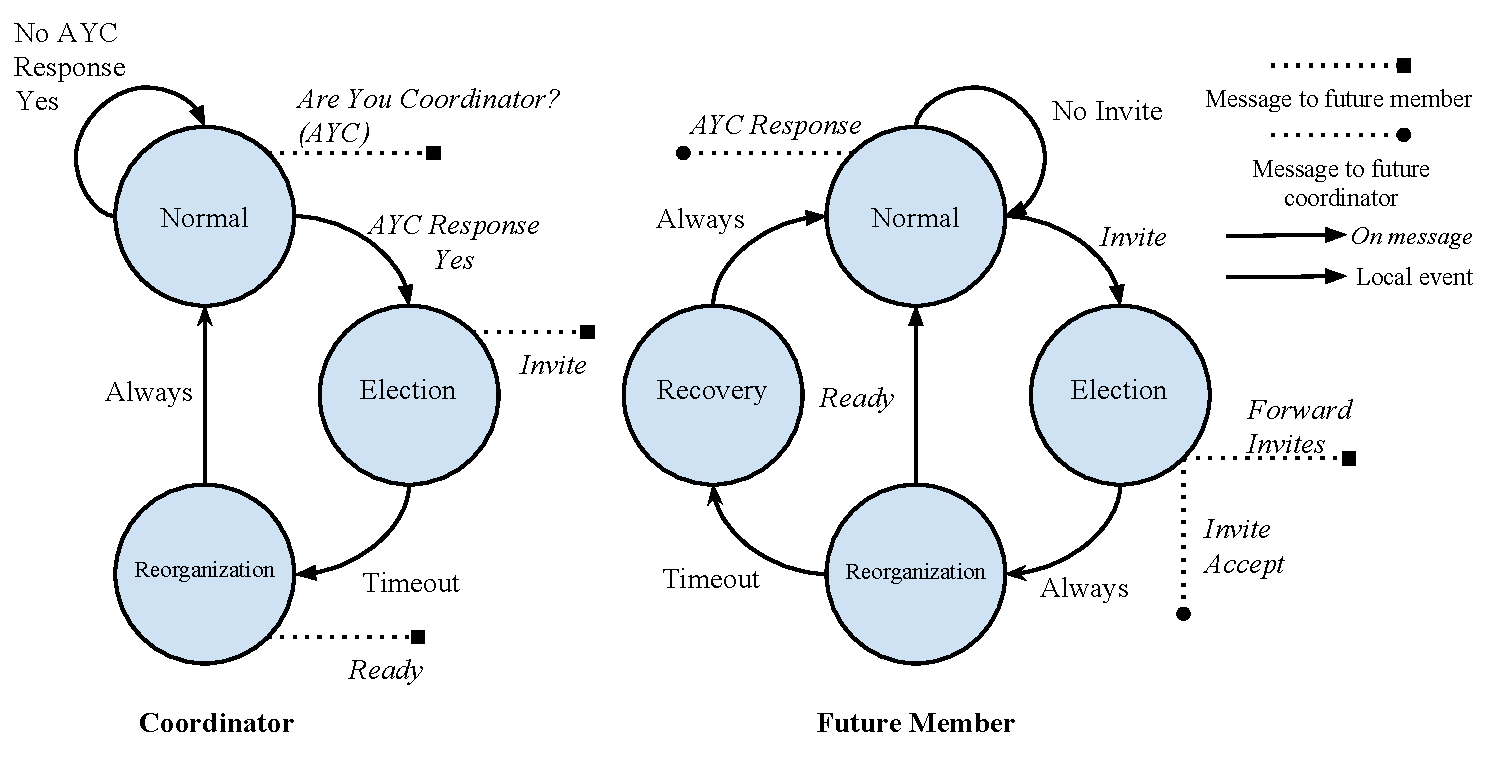
\includegraphics[width=\linewidth]{LeaderElectionStateDiagram.pdf}
\caption{State machine of a leader election. Processes start as coordinators in the ``Normal'' state and search for other coordinators to join with. Processes immediately respond to ``Are You Coordinator'' messages they receive.}
\label{fig:statemachine}
\end{figure*}

Once a group is formed it must be maintained.
To do this, processes occasionally exchange messages to verify the other is still reachable.
This interaction is shown in Figure \ref{fig:statemachine2}.
Coordinators send ``Are You Coordinator'' messages to members of its group to check if the process has left the group.
Group members send ``Are You There'' messages to the coordinator to verify they haven't been kicked out of the group, and to ensure the coordinator is still alive.
If processes fail to reply to received message before a timeout, they will leave the group.
Leaving the group can either be caused by the coordinator removing the process, or the process can enter a recovery state and leave the group, forming a new group by itself.

\begin{figure*}[!t]
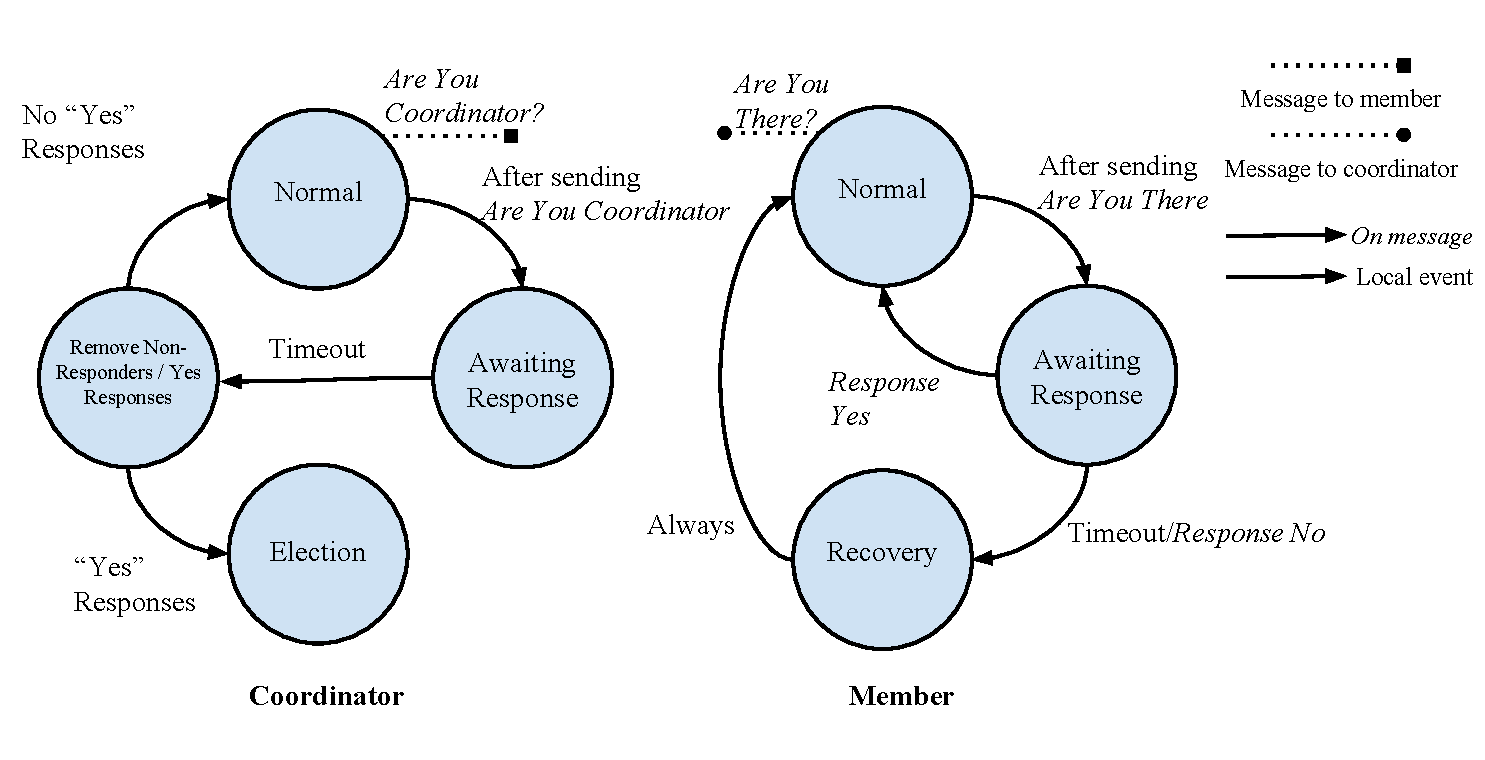
\includegraphics[width=\linewidth]{MaintainStateDiagram.pdf}
\caption{State machine of maintaining a group. The ``Are You Coordinator'' messages are the same as those in Figure \ref{fig:statemachine}. ``Are You Coordinator'' and ``Are You There'' are periodically sent by processes, and responses to those messages are immediately sent by the receiving process.}
\label{fig:statemachine2}
\end{figure*}

For a variety of reasons modeling this algorithm is very difficult.
Previous work, \cite{CRITIS2012}, showed data collected of an implementation of the algorithm display have a large amount of variance.
In a distributed system information cannot be instantaneously spread throughout the system.
As a consequence, omission failure will cause a process to miss out on information distributed by other processes.
In particular, the receipt of ``Ready'' messages by group members is uncertain to the coordinator.
This missing information normally causes the coordinators observation of the group to be out-of-date.
Since the state of the group is incorrect, it cannot be used with a Markov chain, as it does not describe the actual state of the system.
The original ``Are You There'' approach for detecting failure detection (Figure \ref{fig:statemachine2}) also causes a similar effect.
Additionally, the election algorithm has an inherent race condition as part of its normal operation.
This race condition can make the selection of the group leader inconsistent: the highest priority process may not always win the election.
For the purpose of analyzing the system, having a consistent leader is important for collecting data to verify the model.

In this work, we model what a process will observe as a result of omission failure.
Therefore, it is important a process' observations hold to the Markov property.
The original Garcia-Molina algorithm has been modified so the observations of the coordinator process have the Markov property.
The full modified algorithm is presented in Appendix REFERENCE.
The following sections state the portions of the algorithm where the observation of the leader process does not yield the probability of next transition.
Changes to the algorithm relieved race conditions when selecting a leader, and made the state of the members a certainty for the coordinator.

\subsection{Leader Selection}

To alleviate the inherit race condition of leader selection, a fixed leader process was selected.
This process was the only one that could become the leader of a multiprocess group.
This simplification was applied because the configuration of the system with a larger number of processes depended on the configuration of the other processes.
Without this simplification, the state of the rest of the system would not have the memoryless property.
The state of the processes that are not in the observers group would change each round.
As a consequence the state of the rest of the system and the likelihood of forming a specific group size would change each step if other processes could become leader.
A probabilistic prediction would depend on how long the processes have been separated.
After a long enough period of time the distribution of states for the processes could be found using a steady-state analysis.
However, when processes enters the ``Recovery'' state they are deterministically placed in the alone state.
As a consequence the state of the system depends on the number of steps since the last reconfiguration, which violates the memoryless property.

Suppose P1 fails to detect P2 and P3 multiple times.
The probability P2 has grouped with P3 could then be modeled as a two process sub-case of this three process case.
Let this two process sub-case be described with a profile chain $P_{sub}$.
The probability of P2 and P3 joining P1's group depends on the state of the sub-case.
Additionally the probability distribution of an observation of the sub-case depends how many steps the sub-case has completed.
If $P_{sub}$ is ergodic, then $Steady(P_{sub}{}) \neq [1.0 \quad 0]$.
Each step of the sub-case ($n$) will move its distribution asymptotically closer to the steady-state:

\[ [1.0 \quad 0] * \lim_{n \to \infty}P_{sub}^n = Steady(P_{sub}) \]

Since the initial state of the algorithm in the sub-case must be un-grouped ($[1.0 \quad 0]$), and the process is ergodic, the probability distribution of the sub-case depends on the number of steps ($n$).
As a consequence, the distribution for any $n$ must be different from the distribution of $n-1$.
Since the probability of P1 completing an election of P2 and P3 depends on the grouping of P2 and P3, the behavior of the full case cannot be memoryless, since it is a function of $n$.
Therefore, to make the algorithm memoryless, only a selected process may lead a multiprocess group.

\subsection{Ready Acknowledgment}

The changes added a third message to completing an election -- a ready acknowledge message.
This message is sent by a member after receiving the ready message from the coordinator.
This allows the coordinator to be certain of the member's status before the next round.
Without the ready acknowledgment, the member may not receive the ready message and the coordinator will observe the member is a part of the group.
This interaction is shown in Figure \ref{fig:lostready}.

\begin{figure}
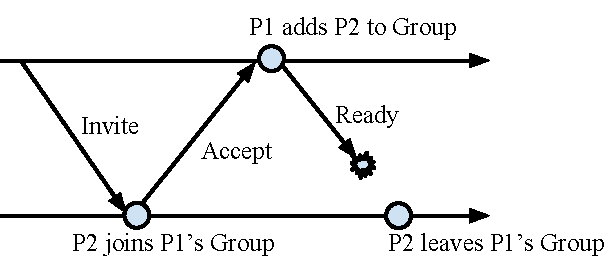
\includegraphics[width=\linewidth]{LostReady.pdf}
\caption{The grouping processes effects the outcome of elections} \label{fig:lostready}
\end{figure}

Without the ready acknowledgment message, the probability a member remains in a group in the first round after an election has a different probability than each subsequent round.
By adding the extra message, the observation of the coordinator must be the state of the member of the group.
As a consequence, the probability a member remains in a group in the first round after an election is identical to each subsequent round.

\subsection{Failure Detection}

Members cannot leave a group without the leader's permission.
Members do not suspect the coordinator has failed, only the coordinator may suspect the members.
For the purpose of starting an election, an ``Are You There'' message and its negative response are considered equivalent to a ``Are You Coordinator'' message and a positive response.
On receipt of the negative response, the member will immediately recover and become a leader.
This assumption relies on ``Are You Coordinator'' and ``Are You There'' messages being sent at roughly the same time.
This change leads to a live-lock situation in a crash failure, where the group's leader crashes and does not return and as a consequence the remaining members are trapped in a group without a leader.
For the purpose of this work, we have disregarded these live lock scenarios.


\subsection{Creation of A Profile Chain}

The election algorithm produces and distributes a set of processes $UpPeers$ and a coordinator of that set.
$UpPeers$ is distributed via message passing and maintained by the coordinator.
Different processes may have different versions of $UpPeers$ for a given coordinator as processes enter and leave the group.
However, a process will eventually receive an up-to-date version of $UpPeers$ from the coordinator, or it will leave the group.

To model the behavior of the algorithm, at each time-step the selected process recorded the cardinality of its membership set $UpPeers$.
The selected process was always the coordinator of any formed group, and was the only process that could lead a multi-process group.
The cardinality of $UpPeers$ directly mapped to the state in the Markov Chain.
For example given the membership set $S=\{P1,P2,P3\}$, then $\left | S \right |=3$ and the state of the system in the Markov chain is also $i=3$.

The profile Markov chain for the algorithm was constructed as a closed form representation of the algorithm's behavior.
Each round, the behavior is described by two components: maintaining a group and inviting other processes into the group.
The coordinator will exchange a ``Are You Coordinator'' message and the peer will respond to verify is still available.
To maintain a group of $m$ other processes, the probability is defined as a random variable with the following probability distribution (pdf):

\[
 \Pr_{M}(X=k; m) =
   \begin{cases}
    \binom{m}{k} p^{2k}(1-p^2)^{m-k} & \quad \text{if } 0 \leq k \leq m \\
    0                                & \quad \text{otherwise} \\
  \end{cases}
\]

Where $k$ is the number of processes remaining in a group selected from $m$ processes.
A process will leave a group if, from the considered process' perspective, they do not respond to an ``Are You Coordinator'' message.
Members cannot change their state without coordinating with the leader.

To invite other processes to the group, the two processes ultimately exchange up to 8 messages.
In a round, a single process can invite many other processes to its group.
From a selection of $n$ other coordinators, the probability distribution for joining a new group with $k$ of the $n$ processes is:

\[
	\Pr_{I}(Y=k; n) =
	\begin{cases}
		\binom{n}{k} p^{8k}(1-p^8)^{n-k} & \quad \text{if } 0 \leq k \leq n \\
		0                                & \quad \text{otherwise} \\
	\end{cases}
\]

In the profile chain, in a state $s$ that describes the number of processes in a group, the probability of transitioning from $s$ to $s'$ with $n$ total processes (including the considered process) is:

\[ \Pr_{T}(Z=s'; n; s) = \sum_{i=0}^{s-1} \Pr_{M}(X=i; s-1) \Pr_{I}(X=s'-i; n-s-1) \]

From this distribution, a set of transition probabilities can be calculated for a given omission rate $p$ and number of processes $n$.
This set of transition probabilities forms a profile Markov chain $P$, which can be evaluated to for any number of processes $n$ and omission rate $p$.
The generated profile chain is ergodic when $0<p<1.0$. The profile chain is a stationary Markov chain.

%State that the profile chain is stationary. State a that a test input sequence is the realization of a run of a system as a Markov chain T. State that we generate test matrices for sequences of input chains.
%State what the test chainge means for a run of the DGI. explain how the chain is extracted (maximum likelihood estimates aka the obvious way)
% sampling the test chains

\section{Creating a Test Chain of Implemented Algorithm}

To verify the profile chain describes the behavior of the algorithm, it must be compared to the algorithm.
By constructing a test chain from the execution of the algorithm, we can verify the profile chain describes the algorithm.
The test chain, $T$, is constructed by executing the algorithm in the DGI environment and recording a process's observations of group size.
The implementation of the election algorithm was executed for a sufficient number of steps to collect observations to estimate the transition matrix $T$.
Data was collected by running an implementation of the algorithm in the DGI software\ref{FREEDMGITHUB}.
Each process ran on its own Intel Core 2 Duo E4600 CPU, running Debian GNU/Linux 7.8 (wheezy) and the 3.2.65 RT kernel.
Computers connected on a gigabit network with clocks synchronized by NTP, and a fine synchronization technique used in the DGI.
DGI was compiled with Boost\cite{BOOST} 1.49 and Google's Protocol Buffers\cite{PROTOBUF} 2.4.1.
Messages were sent as UDP Datagrams and dropped by the receiver based on a Bernoulli trial from the Boost library.
For each test-case the DGI was run for 5,000 time-steps to collect a sufficient number of observations.
The collected observations form a sequence of states.
A transition probability matrix can be extracted from that sequence, using a maximum likelihood estimates approach.
Let $n_{ij}$ be the number of observed transitions from state $i$ to state $j$. Let $n_{i}=\sum_{j=1}^{m} n_{ij}$ where $m$ is the number of states.
The transition probability for each transition in the test matrix $T$ can be written as:

\begin{equation} T_{ij} = \frac{n_{ij}}{n_{i}}. \end{equation}

%State that verification of the profile chain via statistical tests is important. State that if P and T are ergodic stochastic sources and can generate similar sequences if they have the same transition probabilities. State that statistical tests can identify if two chains are different at some significant level. 
%State the hypotheis of the test. H0 and H1
%State the test.
%State the number from the summation and how the degrees of freedm is calculated. State how the critical value is selected. State how the how test is conducted. State that the resulting data doesn�t allow us to reject H0
%State what rejection would mean. State additional tests are needed to confirm the awesomeness of the chain

\section{Model Validation}

%State that verification of the profile chain via statistical tests is important. State that if P and T are ergodic stochastic sources and can generate similar sequences if they have the same transition probabilities. State that statistical tests can identify if two chains are different at some significant level.

To assert the closed form profile chain accurately represents the implementation of the algorithm, it must be validated.
Since $T$ and $P$ are ergodic, they can be checked for equivalence using a goodness-of-fit test.
If the goodness-of-fit test indicates the chains are equivalent, they will generate similar sequences and have similar properties when analyzed.
Therefore, generated $P$ chains can be used to analyze the behavior of the algorithm during live execution with changing conditions.

To verify the test chain $T$ is equivalent to the profile chain $P$, a $\chi^2$ goodness-of-fit test is employed.
The null-hypothesis of this test ($H_{0}$) asserts the profile chain $P$ is equivalent to the test chain $T$:

\[ H_{0}: T = P \]

With an alternative hypothesis that the two chains are not equivalent:

\[ H_{1}: T \neq P \]

The $\chi^2$ test measures the goodness-of-fit for a complete chain by combining the measurements of goodness of fit for the transitions away from each state.
Therefore, the goodness of fit test for the chain is a summation of tests for each state:\cite{MARKOV3}

\[ \chi^2 = \sum_{i}^{m} \sum_{j}^{m} = \frac{n_{i}(P_{ij}-T_{ij})^2}{P_{ij}} \]

Where $n_{i}$ is the number of times the state $i$ was observed in the input sequence used to construct the test chain $T$.
The summation is distributed as $\chi^2$ with $m(m-1)$ degrees of freedom if all entries in $P_{ij}$ are non-zero.
In this work, all transitions in the profile Markov chain $P$ are non-zero when $0<p<1.0$.
However, the probability of some transitions may be extremely small.
The $\chi^2$ value was compared to a critical value (CV) giving a measure of how likely it was $H_{0}$ could not be rejected.
This work selected an $\alpha = 0.05$ significance level to accept the hypothesis $T=P$.

If the hypothesis $H_{0}$ were to be rejected, it would indicate the test chain and profile chain differ significantly.
As a consequence of rejecting the hypothesis, the implementation would have behavior from the generated closed form solution.

To verify the model, it was compared to runs of an implementation of the algorithm.
Test data was collected for systems with 3, 4, 5 and 6 processes.
Information was collected from sufficiently long runs of the system with an omission rates between 0.05 and 0.95 tested at intervals of 0.05.
Table \ref{tab:chisummary} shows the measured error and p-value for the worst observed error for each number of processes.
Since the measured error is less than the critical value and the p-value is greater than 0.05, the profile chains ($P$) are representative of the behavior of the algorithm's implementation.

\begin{table*}[!t]
\centering
\begin{tabular}{ c | c c c c c}
  \hline
  Processes & Degrees of Freedom & Critical Value (CV) & Worst Error & $\Pr(WorstError)$ &  p-value \\ \hline
  3 & 6 & 12.6 & 8.90 & 0.80 & 0.18 \\
  4 & 12 & 21.0 & 14.55 & 0.75 & 0.27 \\
  5 & 20 & 31.4 & 23.47 & 0.65 & 0.27 \\
  6 & 30 & 43.8 & 32.69 & 0.85 & 0.34 \\
\end{tabular}
\caption{Summary of $\chi^2$ tests performed.}
\label{tab:chisummary}
\end{table*}

% State the application of the profile chain
% Describe the in group time measure and why it is relevant.
% Embed tables of the steady state over time
% Highlight critical points, discuss the shape of the curve?
% Mention how an invariant could be applied to adjust the schedule to improve the IGT by increasing P.
% Make a quality of service argument?

\section{Profile Chain Applications}


The DGI focuses on managing power resources in a microgrid environment.
Resources can only be managed effectively when multiple DGI coordinate together to manage those resources.
Without another DGI to coordinate with, the DGI has a limited range of options to manage power generation, storage and loads.
Therefore, the amount of time DGI will spend coordinating with another process is of particular interest.
\cite{CRITIS2012} defines an ``In Group Time'' (IGT) metric to measure the amount of time a DGI process spends coordinating with at least one other process.
In this work, we define IGT based on the steady state of the profile chain.
Let $\pi=Steady(P)$ for some profile chain.
The IGT is the sum of all states in $\pi$, save the first state where the process is alone:

\[ IGT = \sum_{i=2}^{m} \pi_i \]

The IGT is a number between 0 and 1.
It represents the probability a random observation sees a group of at least two members.
The steady state distributions are presented as stacked bar graphs in Figures \ref{fig:3process}, \ref{fig:4process}, \ref{fig:5process} and \ref{fig:6process}.
Each complete bar in the graph indicates the IGT.
The components of each bar represent the probability the system is in a specific state for a random observation of the system.
The height of the component represents the relative probability of observing that state when in a group.

\begin{figure}
    \centering
    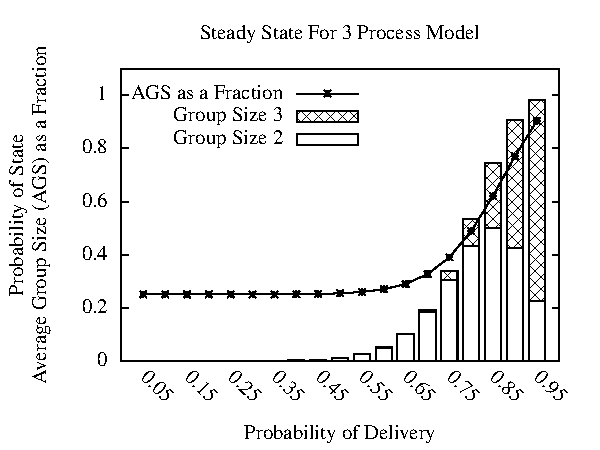
\includegraphics[width=0.65\textwidth]{ss-3process.pdf}
    \caption{Steady state distribution for 3 processes.}
    \label{fig:ss-3process}
\end{figure}

\begin{figure}
    \centering
    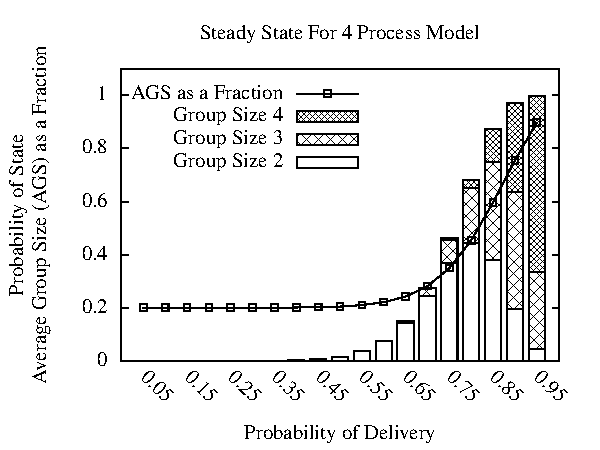
\includegraphics[width=0.65\textwidth]{ss-4process.pdf}
    \caption{Steady state distribution for 4 processes.}
    \label{fig:ss-4process}
\end{figure}

\begin{figure}
    \centering
    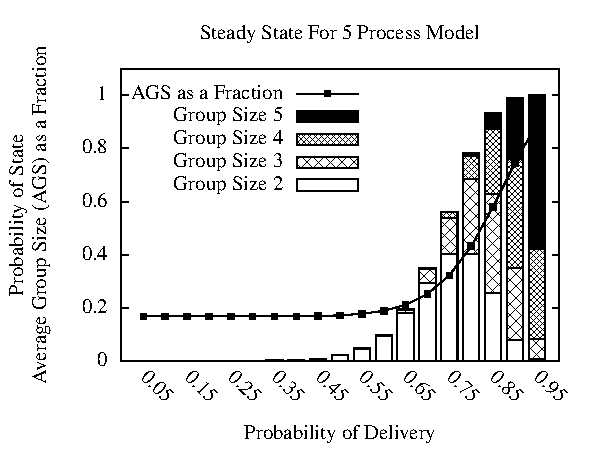
\includegraphics[width=0.65\textwidth]{ss-5process.pdf}
    \caption{Steady state distribution for 5 processes.}
    \label{fig:ss-5process}
\end{figure}

\begin{figure}
    \centering
    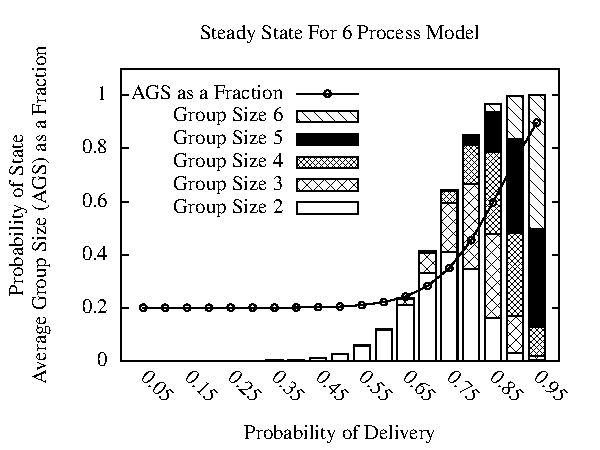
\includegraphics[width=0.65\textwidth]{ss-6process.pdf}
    \caption{Steady state distribution for 6 processes.}
    \label{fig:ss-6process}
\end{figure}

The profile chain can be used to ensure the FREEDM smart-grid is able to continue operating despite network issues.
The profile chain can be combined with different message sending strategies to maintain service.
For example, the DGI can change to a slower mode of operation to ensure operation continues normally despite connectivity issues.
By selecting different strategies depending on the message delivery probability the DGI can offer high performance in good network conditions and an acceptable level of service during faults.




% Write words and things

\section{Conclusion}

In this work we presented a new approach to modeling the behavior of a distributed algorithm.
By modifying the algorithm so the observations of a process are memoryless, the system can be modeled as Markov chain.
These changes do limit the capabilities of the algorithm.
Only one process can lead groups, and the algorithm could live-lock in the event of a crash-failure of the selected process.
However, it does establish a new approach to designing distributed algorithms.
These models accurately represent the behavior of the algorithm during omission failures.
Steady-state analysis of these models yields predictions for how much time a group can spend working.
This measured "In Group Time" can be used to adjust the schedule of a real-time system using the algorithm to ensure it can continue to do work.
Using this adjusting schedule approach the robustness of a cyber-physical system can be enhanced.






% if have a single appendix:
%\appendix[Proof of the Zonklar Equations]
% or
%\appendix  % for no appendix heading
% do not use \section anymore after \appendix, only \section*
% is possibly needed

% use appendices with more than one appendix
% then use \section to start each appendix
% you must declare a \section before using any
% \subsection or using \label (\appendices by itself
% starts a section numbered zero.)
%


\appendices
\begin{algorithmic}

\State $AllPeers \gets \{ 1, 2, ..., N \}$
\State $Coordinators \gets \emptyset$
\State $UpPeers \gets { Me }$
\State $State \gets Normal$
\State $Coordinator \gets Me$
\State $Responses \gets \emptyset$
\State $Counter \gets$ A random initial identifier
\State $GroupID \gets (Me,Counter)$

\State

\Function{Check}{}
    \State This function is called at the start of a round by the leader
    \If {$State = Normal$ and $Coordinator \gets Me$}
        \State $Responses \gets \emptyset$
        \State $TempSet \gets \emptyset$
        \For {$j = (AllPeers - \{Me\})$}
            \State $AreYouCoordinator(j)$
            \State $TempSet \gets TempSet \cup j$
        \EndFor
        \State Peers which respond "Yes" to $AreYouCoordinator$ are put into the $Responses$ set.
        \State When an $AreYouThere$ response is "No" and this process is a coordinator, the querying process is put in the $Responses$ set.
        \State Wait for $Timeout(CheckTimeout)$, Peers that do not respond are removed from UpPeers.
        \State $UpPeers \gets (TempSet-Responses) \cup {Me}$
        \If {$Responses = \emptyset$}
            \Return
        \EndIf
        \State $p \gets \max(Responses)$
        \If $Me > p$
            \State Wait time proportional to me-p
        \EndIf
        \Call{Merge}{Responses}
    \EndIf
    \State The next call to this is after Timeout(CheckTimeout)
\EndFunction

\State

\Function{Timeout}{}
    \State This function is called at the start of a round by the group members
    \If {$Coordinator = Me$}
        \Return
    \Else
        \Call{AreYouThere}{Coordinator,GroupID,Me}
        \If{Response is No}
            \Call{Recovery}{}
        \EndIf
    \EndIf
    \State The next call to this is after Timeout(TimeoutTimeout)
\EndFunction

\State

\Function{Merge}{Coordinators}
    \State This function invites all coordinators in Coordinators to join a group led by Me
    \State $State \gets Election$
    \State Stop work
    \State $Counter \gets Counter+1$
    \State $GroupID \gets (Me,Counter)$
    \State $Coordinator \gets Me$
    \State $TempSet \gets UpPeers - {Me}$
    \State $UpPeers \gets \emptyset$
    \For {$j \in Coordinators$}
        \Call{Invite}{j,Coordinator,GroupID}
    \EndFor
    \For {$j \in TempSet$}
        \Call{Invite}{j,Coordinator,GroupID}
    \EndFor
    \State Wait for $Timeout(InviteTimeout)$, Peers that accept the invite are added to UpPeers
    \State $State \gets Reorganization$
    \For {$j \in UpPeers$}
        \Call{Ready}{j,Coordinator,GroupID,UpPeers}
    \EndFor
    \State $Acknowledge \gets UpPeers$
    \State Wait for $Timeout(ReadyTimeout)$, Peers that do not acknowledge are removed from UpPeers
    \State $UpPeers \gets UpPeers - Acknowledge$
    \State $State \gets Normal$
\EndFunction

\State

\Function{ReceiveReady}{Sender,Leader, Identifier, Peers}
    \If {$State = Reorganization$ and $GroupID = Identifier$}
        \State $UpPeers \gets Peers$
        \State $State \gets Normal$
        \State Respond Ready Acknowledge
    \EndIf
\EndFunction

\State

\Function{ReceiveAreYouCoordinator}{Sender}
    \If {$State = Normal$ and $Coordinator = Me$}
        \State Respond Yes
    \Else
        \State Respond No
    \EndIf
\EndFunction

\State

\Function{ReceiveAreYouThere}{Sender, Identifier}
    \If {$GroupID = Identifier$ and $Coordinator = Me$ and $Sender \in UpPeers$}
        \State Respond Yes
    \Else
        \State Respond No
        \State Add sender to $Responses$ set for $Check()$ if this process is a coordinator.
    \EndIf
\EndFunction

\State

\Function{ReceiveInvitation}{Sender,Leader,Identifier}
    \If {$State \neq Normal$}
        \Return
    \EndIf
    \If {$Sender \neq 0$}
        \Return
    \EndIf
    \State Stop Work
    \State $Temp \gets Coordinator$
    \State $TempSet \gets UpPeers$
    \State $State \gets Election$
    \State $Coordinator \gets Leader$
    \State $GroupID \gets Identifier$
    \If {$Temp = Me$}
        \State Forward invite to old group members
        \For $j \in TempSet$
            \State $Invite(j,Coordinator,GroupID)$
        \EndFor
    \EndIf
    \State $Accept(Coordinator,GroupID)$
    \State $State \gets Reorganization$
    \If {$Timeout(ReadyTimeout)$ expires before $Ready$ is received}
        \State $Recovery()$
    \EndIf
\EndFunction

\State

\Function{ReceiveAccept}{Sender,Leader,Identifier}
    \If {$State \gets Election$ and $GroupID = Identifier$ and $Coordinator = Leader$}
        \State $UpPeers \gets UpPeers \cup {Sender}$
    \EndIf
\EndFunction

\Function{ReceiveReadyAcknowledge}{Sender}
    \State $Sender$ is removed from $Acknowledge$ in $Merge()$
\EndFunction

\State

\Function{Recovery}{}
    \State $State \gets Election$
    \State Stop Work
    \State $Counter \gets Counter + 1$
    \State $GroupID \gets (Me,Counter)$
    \State $Coordinator \gets Me$
    \State $UpPeers \gets {Me}$
    \State $State \gets Reorganization$
    \State $State \gets Normal$
\EndFunction

\end{algorithmic}




% use section* for acknowledgment
\section*{Acknowledgment}


The authors would like to thank...


% Can use something like this to put references on a page
% by themselves when using endfloat and the captionsoff option.
\ifCLASSOPTIONcaptionsoff
  \newpage
\fi



% trigger a \newpage just before the given reference
% number - used to balance the columns on the last page
% adjust value as needed - may need to be readjusted if
% the document is modified later
%\IEEEtriggeratref{8}
% The "triggered" command can be changed if desired:
%\IEEEtriggercmd{\enlargethispage{-5in}}

% references section

% can use a bibliography generated by BibTeX as a .bbl file
% BibTeX documentation can be easily obtained at:
% http://www.ctan.org/tex-archive/biblio/bibtex/contrib/doc/
% The IEEEtran BibTeX style support page is at:
% http://www.michaelshell.org/tex/ieeetran/bibtex/
%\bibliographystyle{IEEEtran}
% argument is your BibTeX string definitions and bibliography database(s)
%\bibliography{IEEEabrv,../bib/paper}
%
% <OR> manually copy in the resultant .bbl file
% set second argument of \begin to the number of references
% (used to reserve space for the reference number labels box)

\bibliographystyle{IEEEtran}
% argument is your BibTeX string definitions and bibliography database(s)
\bibliography{IEEEabrv,latex_bibliography}


% biography section
% 
% If you have an EPS/PDF photo (graphicx package needed) extra braces are
% needed around the contents of the optional argument to biography to prevent
% the LaTeX parser from getting confused when it sees the complicated
% \includegraphics command within an optional argument. (You could create
% your own custom macro containing the \includegraphics command to make things
% simpler here.)
%\begin{IEEEbiography}[{\includegraphics[width=1in,height=1.25in,clip,keepaspectratio]{mshell}}]{Michael Shell}
% or if you just want to reserve a space for a photo:


\begin{IEEEbiography}[{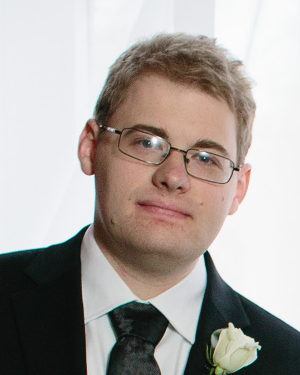
\includegraphics[width=1in,height=1.25in,clip,keepaspectratio]{sjackson}}]{Stephen Jackson}
Received a BS in Computer Engineering and Computer Science from Missouri University of Science \& Technology in 2010. He is currently pursuing a PhD in Computer Science at Missouri S\&T. He is a member of the Critical Infrastructure Protection Laboratory at S\&T, and a recipient of the Information-Assurance GAANN fellowship. His research interests include distributed systems, cyber-physical systems, and system reliability.
\end{IEEEbiography}

% if you will not have a photo at all:
\begin{IEEEbiography}[{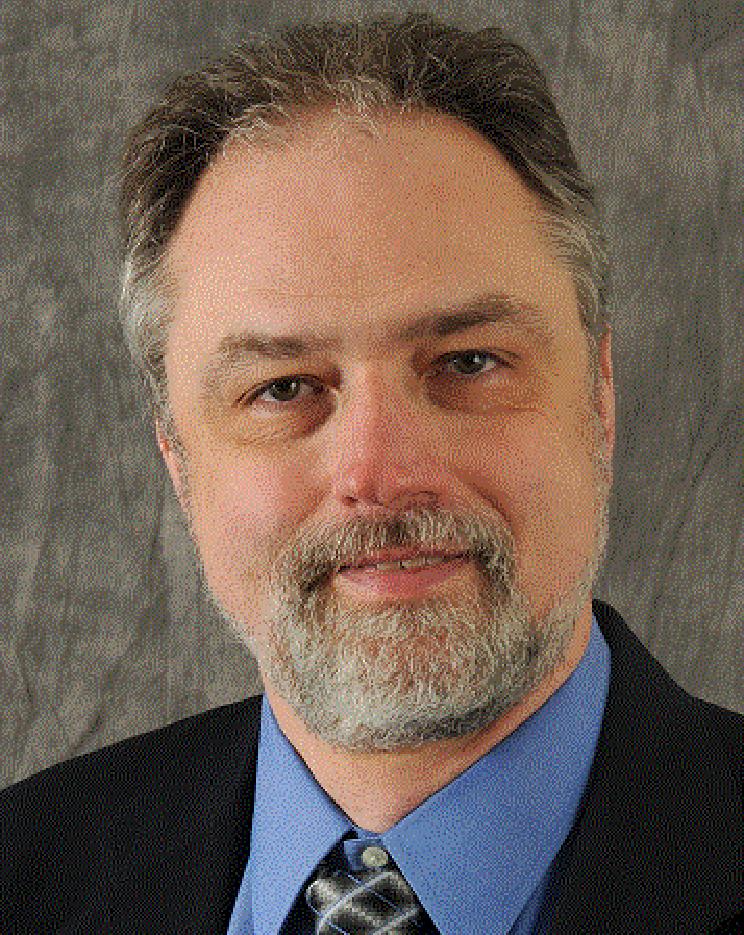
\includegraphics[width=1in,height=1.25in,clip,keepaspectratio]{bmcmillin}}]{Bruce McMillin}
 (SM '07) is currently a Professor
of Computer Science and Director of the Center for
Information Assurance at Missouri S\&T, Rolla, MO,
USA. He leads and participates in interdisciplinary
teams in formal methods for fault tolerance and security
in distributed embedded systems with an eye towards
critical infrastructure protection. He is leading
the distributed grid intelligence project of the Future
Renewables Engineering Research Center.
\end{IEEEbiography}

% insert where needed to balance the two columns on the last page with
% biographies
%\newpage

% You can push biographies down or up by placing
% a \vfill before or after them. The appropriate
% use of \vfill depends on what kind of text is
% on the last page and whether or not the columns
% are being equalized.

%\vfill

% Can be used to pull up biographies so that the bottom of the last one
% is flush with the other column.
%\enlargethispage{-5in}



% that's all folks
\end{document}


